\documentclass[11pt]{article}

\usepackage[utf8]{inputenc} % Required for inputting international characters
\usepackage[T1]{fontenc} % Output font encoding for international characters
\usepackage{booktabs}
\usepackage{mathpazo} % Palatino font
\pretolerance=150
\usepackage{amsmath}

\begin{document}

%----------------------------------------------------------------------------------------
%	TITLE PAGE
%----------------------------------------------------------------------------------------

\begin{titlepage} % Suppresses displaying the page number on the title page and the subsequent page counts as page 1
	
	\center % Centre everything on the page
	
	%------------------------------------------------
	%	Headings
	%------------------------------------------------
	
	\textsc{\LARGE SVEU\v{C}ILI\v{S}TE U ZAGREBU}\\[0.4cm] % Main heading such as the name of your university/college
	\textsc{\LARGE \textbf{FAKULTET ELEKTROTEHNIKE I RA\v{C}UNARSTVA}}\\[2.5cm]
    
	\textsc{\Large Projekt iz Bioinformatike}\\[0.5cm] % Major heading such as course name
	

	%------------------------------------------------
	%	Title
	%------------------------------------------------
	
	
	{\huge\bfseries Ra\v{c}unanje najduljeg zajedni\v{c}kog prefixa temeljeno na BWT}\\[1.2cm] % Title of your document
	
	
	%------------------------------------------------
	%	Author(s)
	%------------------------------------------------
	\begin{minipage}{2.5\textwidth}
		\begin{flushleft}
			\large
			\textit{Autori}\\
			 \textsc{Zvonimir Jurelinac, Tomislav Živec, Tonko Čupić} % Your name
		\end{flushleft}
	\end{minipage}
	~\\[0.2cm]
	\begin{minipage}{2.5\textwidth}
		\begin{flushleft}
			\large
			\textit{Voditelj}\\
			doc.dr.sc \textsc{Mirjana Domazet- Lo\v{s}o} % Supervisor's name
		\end{flushleft}
	\end{minipage}
	
	% If you don't want a supervisor, uncomment the two lines below and comment the code above
	%{\large\textit{Author}}\\
	%John \textsc{Smith} % Your name
	
	%------------------------------------------------
	%	Date
	%------------------------------------------------
	
	\vfill\vfill\vfill\vfill % Position the date 3/4 down the remaining page
	
	{\large Zagreb, prosinac 2017.} % Date, change the \today to a set date if you want to be precise
	
	%------------------------------------------------
	%	Logo
	%------------------------------------------------
	
	%\vfill\vfill
	%\includegraphics[width=0.2\textwidth]{placeholder.jpg}\\[1cm] % Include a department/university logo - this will require the graphicx package
	 
	%----------------------------------------------------------------------------------------
	
	
\end{titlepage}

%----------------------------------------------------------------------------------------
\newpage

\tableofcontents
\newpage

\section{Uvod}

Bioinformatika je grana znanosti koja usko povezuje biologiju i računarstvo, a ubrzano se razvijala zadnja dva desetljeća. Pojeftinjenje i sve veća dostupnost tehnologije sekvenciranja rezultirale su stvaranjem velikih skupova bioloških podataka. Često se kao zadatak u bioinformatici nameće analiza sekvence genoma.
Pošto su te sekvence predugačke za uobičajenu pohranu i analizu, potrebno je koristiti posebna sufiksna polja i polja najdužeg zajedničkog prefiksa. Cilj projekta je bio implementirati algoritme 1 i 2 iz rada Beller et al. (2013), koristeći gotovu knjižnicu za izgradnju sufiksnog polja. 
Zatim je implementacija testirana sa našom implementacijom stabla valića i njegove funkcije rang. Rješenje je uspoređeno s rezultatima iz studetskog rada Mrčela et al. (2016). Kao ulazni niz koristili smo genom bakterije E. Coli

\newpage

\section{Algoritmi}
U problemima analiza sekvenci vrlo često se javlja potreba za izračunom najduljeg zajedničkog prefiksa (LCP). U tu svrhu koriste sufiksni nizovi koji spremaju u listu spremaju sve moguće sufikse sekvence, od duljine 1 do najdulje. Iz sufiksnog niza dobiva se LCP polje u linearnom vremenu. 
Veliki resursni zahtjevi analize senkvenci DNK nameću zahtjeve za korištenjem podatkovnih struktura koje koriste manje memorijskog prostora. Iz te potrebe razvijeno je stablo valića niza transformiranog Burrows- Wheelerovom transformacijom (BWT).
Metoda je sljedeća: sekvenca se prvo podliježe Burrows- Wheelerovoj transformaciji, potom se transformirana sekvenca sprema u stablo valića. Stablo valića podržava pretraživanje unatrag po originalnom nizu pa tako dobivamo tražene sufikse. Opisani algoritam ima složenost $O(n\log\sigma)$, gdje je $\sigma$ veličina abecede.

\subsection{Podatkovne strukture}

\subsubsection{Sufiksno polje}
Sufiksno polje sadrži sve sufikse od teksta S. Zamijenila je u toj zadaći sufiksno stablo jer koristi manje memorije od sufiksnog stabla za istu zadaću. Sufiksno polje se pokazalo kao vrlo važan alat u raspoznavanju i analizi teksta, bioinformatici i drugim primjenama. 
Sufiksno polje SA od niza znakova S je cjelobrojno polje u intervalu od 1 do n koje određuje leksikografski poredak svih n sufiksa niza znakova S. Preciznije, sufiksno polje zadovoljava $ S_{SA[1]} < S_{SA[2]} < ... < S_{SA[n]}$, gdje $ S_i $ označava i-ti sufiks niza znakova S, te sadrži znakove S[i..n].
 
\subsubsection{Burrows- Wheelerova transformacija (BWT)}
\label{BWT_definicija}
Burrows- Wheelerova transformacija pretvara niz znakova u sličan niz znakova BWT[1..n] sa istom abecedom. Koristi se za kompresiju podataka. Transformacija je reverzibilna bez dodatnih resursnih zahtjeva. Elemente transformiranog niza računamo formulom:

\[
BWT[i]=\begin{cases}
S[SA[i]-1], & \text{ako } SA[i]\neq 1 & 
\$, & \text{inače}.
\end{cases}
\]
 
 
\begin{table}
	\caption{Pridruživanje indeksa sufiksima niza S, počevši od najduljeg.}
	\label{tablePrimjer1}
	\begin{center}
		\begin{tabular}{ll}
			\toprule
			i & S$_{SA}$[i] \\
			\midrule
			1 & abrakadabra\$ \\
			2 & brakadabra\$ \\
			3 & rakadabra\$ \\
			4 & akadabra\$ \\
			5 & kadabra\$ \\
			6 & adabra\$ \\
			7 & dabra\$ \\
			8 & abra\$ \\
			9 & bra\$ \\
			10 & ra\$ \\
			11 & a\$ \\
			12 & \$ \\
			\bottomrule
		\end{tabular}
	\end{center}
\end{table}

\begin{table}
	\caption{Sufiksi su poredani leksikografski, a njihovi indeksi čine sufiksno polje SA.}
	\label{tablePrimjer2}
	\begin{center}
		\begin{tabular}{rrll}
			\toprule
			i & SA[i] & S$_{SA}$[i] & BWT[i] \\
			\midrule
			1 & 12 & \$ & a\\
			2 & 11 &  a\$ & r \\
			3 & 8 & abra\$ & d \\
			4 & 1 & abrakadabras\$ & \$ \\
			5 & 6 & adabra\$ & k \\
			6 & 4 & akadabra\$ & r \\
			7 & 9 & bra\$ & a\\
			8 & 2 & brakadabra\$ & a\\
			9 & 7 & dabra\$ & a \\
			10 & 5 & kadabra\$ & a\\
			11 & 10 & ra\$ & b \\
			12 & 3 & rakadabra\$ & b\\
			\bottomrule
		\end{tabular}
		
	\end{center}
	
\end{table}

\newpage

\subsubsection{Stablo valića}
\label{WT_defincija}

Stablo valića je struktura podataka koja rekurzivno particionira tok u 2 dijela sve dok su u svakom dijelu preostali homogeni podatci. Ime stabla je analogno valnoj transformaciji signala koji rekurzivno dekompresira signal prema frenkvencijama komponenti. 

Stablo valića može efikasno raditi upite rank i select nad nizovima proizvoljnih abeceda. To nam omogućuje pretraživanje unatrag u vremenskoj složenosti od  $O(\log\sigma)$ po koraku.
Prvo definiramo uzlazno poredanu abecedu $\Eta$kao niz znakova veličine $\sigma $.  
Zatim definiramo interval [1..r] kao podinterval abecede, r <= $\sigma$
Za interval [1..r], niz znakova BWT[1..r] dobijemo tako da iz transformiranog niza znakova od S uklonimo sve znakove iz B-W transformacije koji ne pripadaju segmentu abecede [1..r]

\section{Primjer rada algoritma}
U nastavku dokumenta dan je primjer rada algoritma na stringu S = mississippi.

\subsection{Izgradnja sufiksnog polja}
\begin{enumerate}
\item Na kraj ulaznog niza dodaje se znak \$ te je sada S =  mississippi\$. U daljnjem tekstu vrijedi pretpostavka da je znak \$ abecedno manji od svih ostalih znakova od kojih je S izrađen.
\item Svakom sufiksu niza S pridružuju se indeksi od 1 do \textit{n}, počevši od najduljeg. Ovo je prikazano u \textbf{tablici \ref{tableEx1}}

\begin{table}
\caption{Pridruživanje indeksa sufiksima niza S}
\label{tableEx1}
\begin{center}
\begin{tabular}{ll}
\toprule
i & S$_{SA}$[i] \\
\midrule
1 & mississippi\$ \\
2 & ississippi\$ \\
3 & ssissippi\$ \\
4 & sissippi\$ \\
5 & issippi\$ \\
6 & ssippi\$ \\
7 & sippi\$ \\
8 & ippi\$ \\
9 & ppi\$ \\
10 & pi\$ \\
11 & i\$ \\
12 & \$ \\
\bottomrule
\end{tabular}
\end{center}
\end{table}

\item Sufiksno polje \(SA\) dobivamo soritiranjem dobivenih sufiksa leksikografski od najmanjeg prema najvećem. Ovo je prikazano u \textbf{tablici \ref{tableEx2}}.

Dobiveno je sufiksno polje SA = [12, 11, 8, 5, 2, 1, 10, 9, 7, 4, 6, 3]

\begin{table}
\caption{Sufiksi su poredani leksikografski, a njihovi indeksi čine sufiksno polje SA.}
\label{tablePrimjer2}
\begin{center}
\begin{tabular}{rrl}
\toprule
i & SA[i] & S$_{SA}$[i] \\
\midrule
1 & 12 & \$ \\
2 & 11 &  i\$ \\
3 & 8 & ippi\$ \\
4 & 5 & issippi\$ \\
5 & 2 & ississippi\$ \\
6 & 1 & misssissippi\$ \\
7 & 10 & pi\$ \\
8 & 9 & ppi\$ \\
9 & 7 & sippi\$ \\
10 & 4 & sissippi\$ \\
11 & 6 & ssippi\$ \\
12 & 3 & ssissippi\$ \\
\bottomrule
\end{tabular}
\end{center}
\end{table}

\item Izračunava se Burrows-Wheelerova transformacija BWT[1..n] za dobiveno sufiksno polje SA prema formuli navedenoj u \ref{BWT_defincija} .  
\newline Npr. BWT[4]=S[SA[4]-1]=S[5-1]=S[4]=s.

Rezultat je prikazan u tablici \textbf{tablice \ref{tableEx3}}. 

\begin{table}
\caption{Burrows-Wheelerova tranformacija}
\label{tableEx3}
\begin{center}
\begin{tabular}{rrll}
\toprule
i & SA[i] & S$_{SA}$[i] & BWT[i] \\
\midrule
1 & 12 & \$ & i \\
2 & 11 &  i\$ & p \\
3 & 8 & ippi\$ & s \\
4 & 5 & issippi\$ & s \\
5 & 2 & ississippi\$ & m \\
6 & 1 & misssissippi\$ & \$ \\
7 & 10 & pi\$ & p \\
8 & 9 & ppi\$ & i \\
9 & 7 & sippi\$ & s \\
10 & 4 & sissippi\$ & s \\
11 & 6 & ssippi\$ & i \\
12 & 3 & ssissippi\$ & i \\
\bottomrule
\end{tabular}
\end{center}
\end{table}

\item Iz dobivene Burrows-Wheelerove transformacije gradi se stablo valića opisanom u \ref{WT_definicija}. Prvo se stvara sortirana abeceda ulaznog niza koja je u ovom slučaju veličine 5 znakova ($\Sigma$[1..5]=\$imps). Korijen stabla čini bit vektor dobiven kodiranjem niza Burrows-Wheelerove transformacije dobivene u prethodnom koraku. Abeceda se potom dijeli na pola te dobivamo dva podniza, ovom slučaju: $\Sigma$[1..2]=\$i i $\Sigma$[3..5]=mps. Znakovi prve polovice u svakoj skupini kodiraju se vrijednošću 0, a ostali 1. Postupak se ponavlja sve dok se u čvoru ne nalaze samo jednaki znakovi koji čine listove stabla. Potpuno izgrađeno stablo za dani primjer prikazano je na slici \ref{fig:waveletTree}.

\begin{figure}
	\begin{center}
		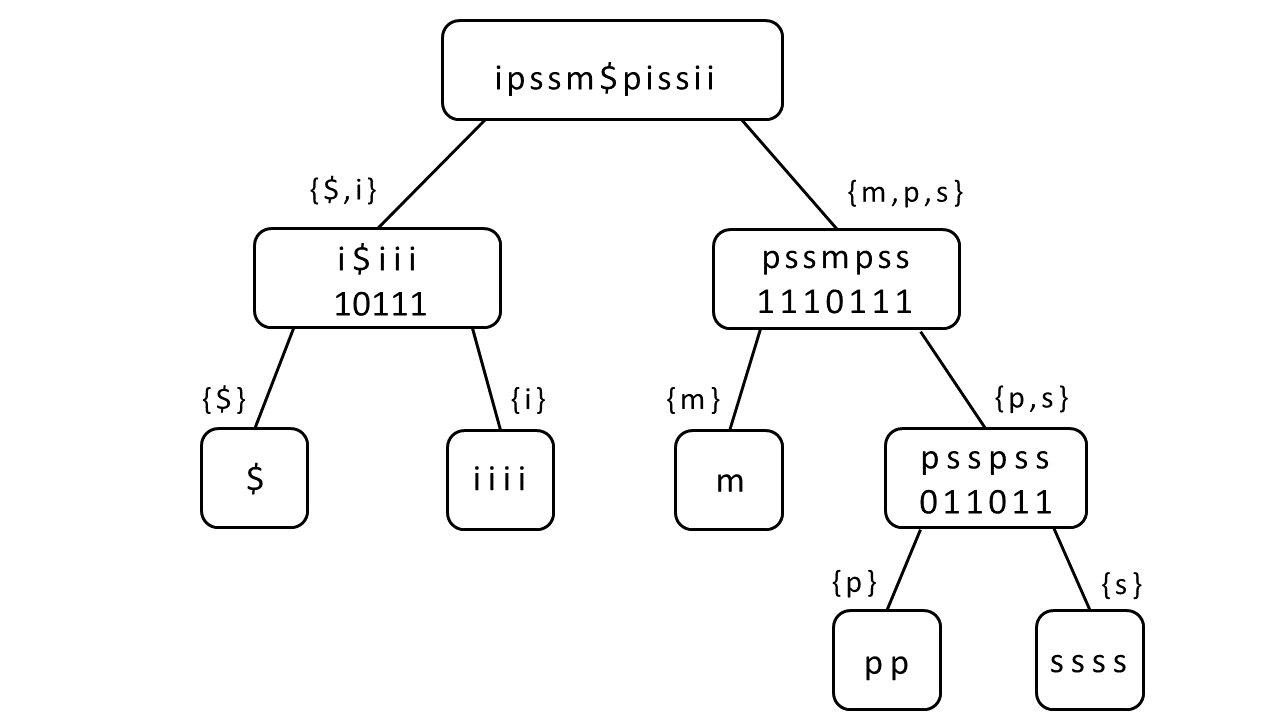
\includegraphics[width=\columnwidth]{waveletTree.png}
		\caption{Stablo valića za dani primjer}
		\label{fig:waveletTree}
	\end{center}
\end{figure}

\item Pomoću Algoritama 1 i 2 iz rada Beller et al. (2013) gradi se polje najdužih zajedničkih prefiksa (LCP) u nekoliko koraka:
  \begin{enumerate}
  \item Inicijalizacija LCP polja i reda Q. Vrijednosti polja LCP se postavljaju na nevažeću (\textbf{NULL}) vrijednost, osim LCP[1] i LCP[n+1] koji se postavljaju na -1. U red Q stavljamo strukturu koja sadrži početni interval $I$ = [i..j]=[1..12] i broj \textit{l}=0 :
  \begin{itemize}
 	LCP = [-1,$\perp,\perp,\perp,\perp,\perp,\perp,\perp,\perp,\perp,\perp,\perp,\perp, \perp$, -1]
	 Q = [<[1..12],0>]
   \end{itemize}
   \item Izračunavanje c$\omega$-\newline intervala za interval dobiven uzimanjem elementa iz reda Q (FIFO) unutar funkcije \textit{getIntervals} iz Algoritma 1 Beller et al. (2013).
   \begin{itemize}
    \item [\textit{c} - znak
    \item [\textit{C[c]} - zbroj rangova svih elemenata leksikografski sortirane abecede koji su manji od c
    \item [\textit{i} - početak intervala
    \item [\textit{j} - kraj intervala
   \item Funkcija \textit{rang(a,k)} vraća broj pojavljivanja znaka \textit{a} do \textit{k}-tog indeksa u polju. 
   \item Znakovi abecede iz intervala $I$ se sortiraju od najmanjeg prema najvećem. Ima onoliko c$\omega$-intervala koliko je i jedinstvenih znakova. Kako je abeceda za dani primjer $\Sigma$[1..5]=\$imps, traži se 5 c$\omega$-intervala.
    \item [$C$ = [0,1,5,6,8]
   \item Indeks početka intervala dobiva se po formuli \textit{rang}(c,i-1)+C[c]+1
\indent Indeks kraja intervala dobiva se po formuli C[c]+\textit{rang}(c,j).
   \item U intervalu $I$ se nalaze svi znakovi abecede (\$,i,m,p,s). Za svaki od znakova računa se njegov interval prema formuli navedenoj iznad.
   \item [\textit{rang}('\$',0)+C['\$']+1..C['\$']+\textit{rang}('\$',12)]=[0+0+1..+0+1]=[1..1]
   \item [\textit{rang}('i',0)+C['i']+1..C['i']+\textit{rang}('i',12)]=[0+1+1..+1+4]=[2..5]
   \item [\textit{rang}('m',0)+C['m']+1..C['m']+\textit{rang}('m',12)]=[0+5+1..+5+1]=[6..6]
   \item [\textit{rang}('p',0)+C['p']+1..C['p']+\textit{rang}('p',12)]=[0+6+1..+6+2]=[7..8]
   \item [\textit{rang}('s',0)+C['s']+1..C['s']+\textit{rang}('s',12)]=[0+8+1..+8+4]=[9..12]
   \item Povratna vrijednost \textit{getIntervals}, prema tome, je lista c$\omega$-intervala: [[1..1],[2..5],[6..6],[7..8],[9..12]]
   \item Za svaki od dobivenih intervala [\textit{lb .. rb}] se potom provjerava vrijednost LCP[\textit{rb}+1]. Ako je vrijednost tog polja \textbf{NULL} u red stavljamo strukturu [<[\textit{lb..rb}],\textit{l}+1>], a na index \textit{rb}+1 vrijednost \textit{l}. Navedeni postupak se ponavlja sve dok u redu ima elemenata, a prva dva koraka prikazana su u nastavku.
	\begin{enumerate}
	\item  
 	LCP = [-1,$\perp,\perp,\perp,\perp,\perp,\perp,\perp,\perp,\perp,\perp, \perp$, -1]
	 Q = [<[1..1],0>]
	[\textit{lb .. rb}] = [1..1], \textit{l} = 0
	\newline LCP[\textit{rb}+1]=LCP[2]=$\perp$ -> u red Q stavljamo strukturu  [<[\textit{lb..rb}],\textit{l}+1>]= [<[\textit{1..1}],1>], a LCP[\textit{rb}+1]=LCP[2]=0.
	\item  
	LCP = [-1,0,$\perp,\perp,\perp,\perp,\perp,\perp,\perp,\perp,\perp, \perp$, -1]
	 Q = [<[2..5],0>,<[1..1],1>]
	[\textit{lb .. rb}] = [2..5], \textit{l} = 0
	\newline LCP[\textit{rb}+1]=LCP[6]=$\perp$ -> u red Q stavljamo strukturu  [<[\textit{lb..rb}],\textit{l}+1>]= [<[\textit{2..5}],1>], a LCP[\textit{rb}+1]=LCP[6]=0.
	\item  
	LCP = [-1,0,$\perp,\perp,\perp,$0$,\perp,\perp,\perp,\perp,\perp, \perp$, -1]
	 Q = [<[6..6],0>,<[2..5],1>,<[1..1],1>]
	[\textit{lb .. rb}] = [6..6], \textit{l} = 0
	\newline (...)
	\end{enumerate}
   \end{itemize}
     \item Vrijednost LCP polja koju dobijemo nakon završetka algoritma je: 
       	LCP = [-1,0,1,1,4,0,0,1,0,2,1,3,-1].
\end{enumerate}

\end{document}